\documentclass[11pt]{article}
\usepackage[margin=1in]{geometry}
\usepackage{times}
\usepackage{natbib}
\usepackage[colorlinks=true,linkcolor=blue,citecolor=blue,urlcolor=blue]{hyperref}
\usepackage{graphicx}
\usepackage{amsmath}
\usepackage{array}
\usepackage{booktabs}
\usepackage{microtype}
\usepackage{url}

\title{\textbf{CSC483/583 Project: Three-Stage Wikipedia Clue Answering}}

\author{
  Cole Mobberly, Suhani Surana, Aunabil Chakma \\
  University of Arizona \\
}

\date{}

\begin{document}

\maketitle

\begin{abstract}
We study Wikipedia clue answering as a retrieval problem: each clue must be mapped to the title of one Wikipedia page. The dataset contains 100 J-Archive clues whose gold answers are Wikipedia titles, and the document collection contains 152,042 indexed non-redirect article pages from a parsed Wikipedia dump. Our system uses a three-stage pipeline. Stage 1 builds a broad candidate list with weighted sparse and dense retrieval. Stage 2 reranks the top 100 candidates with a cross-encoder using natural-question reformulations of the clue. Stage 3 reranks only the top 10 candidates with Qwen3-Reranker-4B. The main result is that answer selection improves when broad retrieval is followed by stronger rerankers over much smaller candidate sets.
\end{abstract}

\section{Introduction}

Wikipedia clue answering is difficult because the clue is often indirect, category-dependent, and phrased differently from the text that appears in the target article. Rather than asking for a direct fact, many clues refer to an entity through paraphrase, role, quoted language, or historical description. This creates a lexical mismatch problem: the words in the clue are often not the words that appear most prominently in the correct Wikipedia page.

We treat the task as page retrieval over Wikipedia. Given a category and clue, the goal is to predict the Wikipedia page title that matches the gold answer. This avoids full generative question answering and turns the task into candidate generation and reranking over 152,042 indexed non-redirect articles. The main challenge is to retrieve the right page despite noisy Wikipedia markup, long article bodies, redirect pages, and clues whose phrasing differs sharply from natural encyclopedia prose.

Our core design principle is to use simpler and cheaper methods early, then apply larger semantic models later only to narrowed candidate sets. The resulting system is a three-stage retrieval pipeline. Stage 1 uses weighted hybrid retrieval, which combines BM25 ranking over cleaned article text with Dense Passage Retrieval (DPR) embeddings \citep{karpukhin-etal-2020-dpr} indexed in FAISS \citep{johnson2019billion}. Stage 2 reranks the top 100 candidates by combining the Stage 1 score with a cross-encoder score from a model trained for passage ranking \citep{nogueira-cho-2019-passage}. Stage 3 exports only the top 10 candidates from Stage 2 and reranks them with Qwen3-Reranker-4B, a larger reranker model \citep{qwen3technicalreport}. We also reformulate each clue into five natural-language questions so that the dense retriever and rerankers see inputs that better match question-versus-passage training distributions. Throughout the paper, Precision@1 (P@1) is the main evaluation metric because the system must return one final Wikipedia title as its answer.

This staged architecture yields consistent gains across the pipeline. Stage 1 reaches a P@1 score of 0.31, Stage 2 improves this to 0.41, and Stage 3 reaches 0.47. These results support a simple conclusion: retrieval quality matters first, but stronger semantic reranking becomes effective once the correct page has been brought into a small candidate set.

\section{Task and Dataset}

Our task is to answer clue-style questions by retrieving the Wikipedia page whose title matches the gold answer. The clues come from J-Archive and follow the Jeopardy clue format, but the system output is not free text: each example contains a category, a clue, and one correct Wikipedia title. This makes the problem a page-ranking task rather than a fully generative question answering task.

We use a dataset of 100 clues whose answers appear as Wikipedia page titles, together with a parsed Wikipedia collection of approximately 280,000 pages. After separating redirects from ordinary articles, we index 152,042 non-redirect article pages. This setup creates two main challenges. First, the collection is large enough that retrieval quality matters immediately. Second, the clues are often indirect and category-dependent, so the wording of the clue may differ substantially from the wording used in the correct Wikipedia article.

\section{Core Implementation}

\subsection{Wikipedia Preprocessing}

We index the collection with Whoosh, treating each Wikipedia page as a separate document rather than indexing one document per source file. This matches the requirement that the final answer must be a Wikipedia page title, so the indexing unit has to be the individual page. We store parsed pages in SQLite, keep redirect pages separate from article pages, and build the retrieval pipeline over page-level article records. In the final system, we index only the non-redirect article pages, which leaves 152,042 indexed documents out of the roughly 280,000 parsed pages.

We also prepared the text specifically for Wikipedia content. In the cleaning stage, we removed redirect lines, section headers, template markup, reference markup, file/image markup, and category lines, then normalized whitespace. Redirect pages were handled explicitly instead of being treated as normal article bodies, because they do not contain meaningful page content and should not be indexed as ordinary evidence-bearing articles in the final system. Instead, the redirect plan was to index redirect titles as aliases and, when a clue matched a redirect title, transfer that score as a boost to the resolved canonical article page.

For term preparation, we tried two paths. The first was a custom normalization pipeline built in our preprocessing code: lowercasing, whitespace tokenization, boundary-punctuation stripping, stop-word removal using spaCy's English stop-word list, removal of non-word characters, and splitting on underscores and hyphens. The second was to index the cleaned article text directly with Whoosh's default analyzer, which applies its own tokenization, lowercasing, stop-word filtering, and stemming. In our experiments, the default Whoosh analyzer was better, so the final system uses that default analyzer rather than the custom tokenized representation.

\subsection{Indexing}
We create multiple sparse and dense indexes so that different evidence sources can be tested inside one weighted retrieval framework. Table~\ref{tab:index-inventory} summarizes the index variants we built.

\begin{table}[t]
  \centering
  \scriptsize
  \caption{Retrieval representations used in the experiments. The first column names the text representation, the second column gives the index backend, and the last column describes what text or embeddings are searched. Except for the body-only baseline, sparse representations use Whoosh's default analyzer.}
  \label{tab:index-inventory}
  \begin{tabular}{p{0.22\linewidth}p{0.08\linewidth}p{0.60\linewidth}}
    \toprule
    \textbf{Representation} & \textbf{Index} & \textbf{Description} \\
    \midrule
    Body text & Whoosh & Sparse retrieval over article body text processed with custom tokenization and normalization. \\
    Title and body text & Whoosh & Sparse retrieval over article titles together with article body text. \\
    Redirect aliases & Whoosh & Sparse retrieval over redirect-page titles, used as alternative names for canonical article pages. \\
    First sentence & Whoosh & Sparse retrieval over only the first sentence of each article. \\
    First two sentences & Whoosh & Sparse retrieval over only the first two lead sentences of each article. \\
    Opening paragraph & Whoosh & Sparse retrieval over only the opening paragraph of each article. \\
    Article categories & Whoosh & Sparse retrieval over Wikipedia category labels linked to each article. \\
    Title with first sentence & FAISS & Dense retrieval using DPR embeddings of the article title plus first sentence. \\
    Title with first two sentences & FAISS & Dense retrieval using DPR embeddings of the article title plus first two sentences. \\
    Title with opening paragraph & FAISS & Dense retrieval using DPR embeddings of the article title plus opening paragraph. \\
    Title with full article & FAISS & Dense retrieval using DPR embeddings of the article title plus full cleaned article text. \\
    Body summary & FAISS & Dense retrieval using DPR embeddings of article-body summaries generated with Qwen. \\
    \bottomrule
  \end{tabular}
\end{table}

Beyond these indexes, we also implemented two simple pattern-based bonuses: one checks whether a four-digit year from the clue also appears in the candidate article, and the other checks whether quoted text from the clue appears in the candidate article. We also tested category-semantic variants, where Wikipedia category labels linked to an article are appended to the dense text representation so that retrieval can use topic labels in addition to article body text. 
Because the clues are often fragments rather than natural questions, we also rewrote each clue into five natural-language questions with Qwen3-8B. 
We used these generated questions as dense-retrieval queries in Stage 1 and as inputs to the later reranking stages. Appendix Figure~\ref{fig:prompt-templates} lists the text templates for inputs and prompts used for our system.

\subsection{Stage 1: Weighted Hybrid Retrieval}

In Stage 1, we build an initial ranking over the full Wikipedia collection using the category text plus the clue text as the query. This stage combines one sparse retrieval score with three dense retrieval scores and is responsible for broad candidate generation before the more expensive rerankers are applied.

For the final selected run, the active Stage 1 components are:

\begin{itemize}
  \item BM25 over custom-processed article body text, weight 15.00
  \item DPR retrieval for the category+clue query, weight 1.00
  \item DPR retrieval averaged over five generated natural questions, weight 1.00
  \item DPR retrieval for the concatenation of those five generated natural questions, weight 1.00
\end{itemize}

Each DPR retrieval score is computed over four dense document indexes: title plus first sentence, title plus first two sentences, title plus first paragraph, and title plus full article text. For a given query, we keep the maximum score returned by these four DPR indexes for each candidate page. In the natural-question mode, we first run DPR separately for each of the five generated questions and then average those candidate scores. We retained title, redirect, lead-only, body-summary, year-based matching, quoted-text matching, and category-semantic dense variants in the codebase, but all of them received zero weight in the final configuration.

This stage gives us a strong but still inexpensive global ranking. It searches the whole collection, surfaces the top candidates for each clue, and supplies the top 100 pages to the cross-encoder stage.

\subsection{Stage 2: Cross-Encoder Reranking}

The second stage reranks the top 100 candidates from the weighted hybrid retriever using a cross-encoder model, \texttt{cross-encoder/ms-marco-MiniLM-L-12-v2} (33M). Each candidate article is represented by its title and cleaned article body, split into 100-token chunks. For each of the five generated natural questions, the system scores all chunks and keeps the best chunk score for that question. The final cross-encoder score for the candidate is the average across the five natural questions. The exact query and document text formats are shown in Appendix Figure~\ref{fig:prompt-templates}.

We then combine the cross-encoder score with the initial Stage 1 score. Both scores are normalized within the top-100 candidate set, and the selected combination uses a weight of 1.00 for the initial score and 7.00 for the cross-encoder score. This combined ranking is Stage 2. It is still local and relatively efficient because it only reads 100 candidates per clue, but it is much more semantically expressive than Stage 1.

\subsection{Stage 3: Qwen3-Reranker-4B}

Stage 3 is an offline reranking experiment performed on the top 10 candidates from the Stage 2 ranking. For each clue, we export the top 10 candidates together with the category, clue, gold answer, five generated natural questions, and a truncated evidence snippet from each candidate article. These exported rows are then scored with Qwen3-Reranker-4B.

We also tried a separate Qwen3-4B chat-model verifier that used a direct yes/no prompt over the same evidence snippets. That approach was not effective as a final ranking method, whereas Qwen3-Reranker-4B, which is a dedicated reranker rather than a chat model, performs much better in the Stage 3 reranking setting (Section~\ref{sec:results}). The exact chat-verifier prompt and reranker input structure are listed in Appendix Figure~\ref{fig:prompt-templates}. Stage 3 cannot recover a correct answer that was not already present in the exported top 10, so it is a pure answer-selection stage rather than a recall-improvement stage.

\begin{figure}[t]
    \centering
    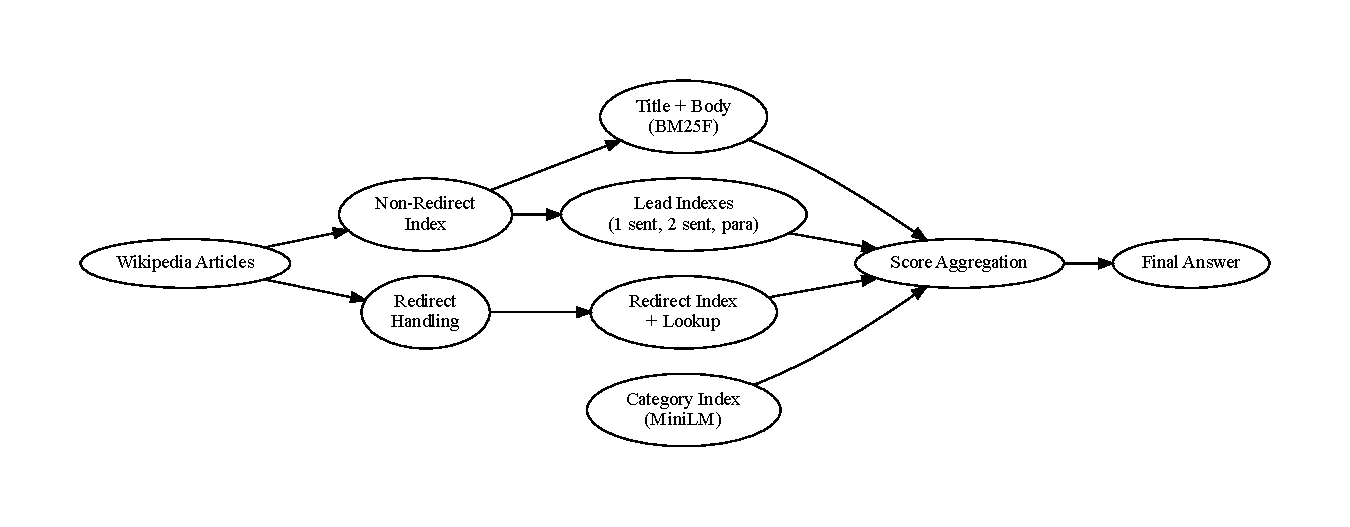
\includegraphics[width=1.0\linewidth]{qa_pipeline.pdf}
    \caption{Final three-stage pipeline. The input category and clue are first mapped to a Stage 1 weighted hybrid ranking over Wikipedia pages. Stage 2 reranks the top 100 pages by combining the Stage 1 score with a cross-encoder score. Stage 3 reranks the top 10 Stage 2 pages with Qwen3-Reranker-4B and returns the highest-ranked title.}
    \label{fig:pipeline}
\end{figure}

\subsection{Compute Environment}

We developed and ran the project across two environments: a local MacBook setup and Google Colab. The local machine was used for the main retrieval codebase, indexing, weight tuning, and most iterative debugging. Google Colab was used for the larger model runs, especially the Qwen-based question generation, summary generation, and reranking experiments.

\subsection{Running the Code}

After installing the Python dependencies with \texttt{pip install -r requirements.txt}, the main 100-question evaluation can be run from the project root with:

\begin{verbatim}
python -m src.run_test_100 --weighted-cole --include-category \
  --cross-encoder --cross-encoder-mode chunks_100 \
  --cross-encoder-query-mode natural_questions_avg \
  --cross-encoder-natural-questions \
  data/processed/questions_natural_qwen3_8b.json
\end{verbatim}

This command evaluates Stage 1 and Stage 2 on the 100-question set and prints the Top-$k$ metrics. For Stage 3, the local code first exports the top 10 Stage 2 candidates:

\begin{verbatim}
python -m src.export_qwen_verifier_inputs \
  --output data/processed/qwen_verifier_inputs.jsonl --top-docs 10
\end{verbatim}

The exported JSONL file is then scored in Google Colab with the Qwen scoring script, using Qwen3-4B for the failed chat-verifier experiment and Qwen3-Reranker-4B for the final Stage 3 reranking. The resulting per-candidate scores are written to \texttt{qwen\_verifier\_scores.jsonl}, and the script prints the Stage 3 Top-$k$ metrics.

\subsection{Implementation Workflow}

We used ChatGPT extensively during implementation to generate code templates, propose project-directory structure, suggest model choices, and help debug basic errors. In particular, it was useful for scaffolding new components quickly, suggesting the cross-encoder reranking approach, surfacing candidate models through search guidance, and helping us think through alternative retrieval designs. We also used it as a consultation tool while deciding how to organize the codebase and which experimental branches were worth implementing.

However, the generated code was not used blindly. We still had to put substantial amount of time reading the generated code carefully, correcting subtle mistakes, and adapting many pieces to the actual behavior of the Wikipedia data and our retrieval pipeline. 
In practice, the LLM assistance reduced implementation time and improved development speed, but it also required manual review and debugging to make the final code correct and coherent.

\section{Evaluation Setup}

As mentioned earlier, we evaluate on the same 100 clues used throughout development, over the final indexed collection of 152,042 non-redirect Wikipedia articles.

The final evaluated system uses the category together with the clue text as the initial query. It first produces a global candidate ranking with the Stage 1 weighted hybrid retriever described in Section 3, then reranks the top 100 candidate pages in Stage 2 by combining the Stage 1 score with the cross-encoder score averaged across five generated natural questions, and finally reranks the top 10 candidates from Stage 2 with Qwen3-Reranker-4B.

We evaluate by normalized title match between the top-ranked predicted page and the gold answer. The primary metric is Precision@1 (Top-1 accuracy), because the system must commit to one final answer. We report Precision@5 as a supporting metric to show whether the correct page is at least being brought near the top of the ranking before the final answer decision.

We directly tuned retrieval weights and selected configurations on the same set of 100 questions used for evaluation. We did not use a separate training or development split, because the dataset is small. As a result, the reported scores should be interpreted as tuned performance on this 100-question set rather than as an unbiased estimate of generalization to unseen clues.

\section{Results and Analysis}

\subsection{Main Results}
\label{sec:results}



\begin{table}[t]
  \centering
  \small
  \caption{Main system-stage comparison on the 100-question set. P@1 measures whether the top-ranked page title is correct, while P@5 shows whether the correct page appears anywhere in the first five results.}
  \label{tab:main-results}
  \begin{tabular}{lcc}
    \toprule
    \textbf{System stage} & \textbf{P@1} & \textbf{P@5} \\
    \midrule
    Sparse body-only baseline, no category & 0.21 & 0.42 \\
    Sparse body-only baseline + category & 0.22 & 0.46 \\
    Stage 1: weighted hybrid retrieval + category & 0.31 & 0.50 \\
    Cross-encoder only & 0.40 & 0.62 \\
    Stage 2: Stage 1 + cross-encoder & 0.41 & 0.61 \\
    Qwen chat verifier & 0.04 & 0.29 \\
    Stage 3: Qwen3-Reranker-4B & \textbf{0.47} & \textbf{0.58} \\
    \bottomrule
  \end{tabular}
\end{table}

Table~\ref{tab:main-results} presents the main system-stage comparison. The largest early gains come from better retrieval. 
The sparse-only baselines reach P@1 scores of 0.21 and 0.22, while the full weighted hybrid configuration reaches 0.31. 
This shows that most of the early improvement comes from stronger candidate generation rather than from later reranking alone.

The cross-encoder then improves answer selection inside the retrieved set. 
Using only the cross-encoder ranking over the top 100 candidates reaches a P@1 score of 0.40, and the full Stage 2 ranking reaches 0.41. 
This suggests that Stage 1 often finds the right page, but because it mainly matches terms instead of meaning, it may not rank that page first.

The final Qwen reranker gives the best Top-1 result, improving the P@1 score from 0.41 to 0.47. 
In count terms, the final system returns the correct page at rank 1 for 47 of the 100 clues. 
This is still a reranking step, like Stage 2, but Qwen3-Reranker-4B is a larger reranker and can make better final distinctions among the strongest candidates. 
However, this gain should be interpreted correctly: Qwen3-Reranker-4B only sees the exported top 10 candidates from the Stage 2 ranking. 
It improves final answer selection inside that top-10 set, but it does not improve recall beyond what earlier stages already retrieved.

The Qwen reranker also lowers P@5 from 0.61 to 0.58, even though P@1 increases. 
This means it is better at placing one answer at the very top, but it does not preserve as many correct answers within the top five. 
Since the main goal is to return a single final answer, the P@1 improvement is the more important result.

One negative result is also important. The Qwen chat verifier performs very poorly, reaching only a P@1 score of 0.04. 
A yes/no chat probability is therefore not a useful final ranking signal for this task, even when the underlying model is much larger than the cross-encoder. 
This setup also does not use a dedicated reranking model or ask the model to answer the clue in one shot. 
More explicit reasoning might improve the chat-based result, but it would also make retrieval slower, which is not ideal for an IR system where fast ranking is important.

\subsection{Grouped Category Analysis}

To make the category-level behavior interpretable, we group the 30 original clue categories into 7 super-categories. Entertainment categories whose answers are mainly people are included under \textit{People}, and business categories are grouped with organizations. Table~\ref{tab:grouped-categories} shows Top-1 counts at each stage.

\begin{table}[t]
  \centering
  \scriptsize
  \caption{Top-1 correct counts by super-category. The examples column shows representative original categories, $N$ is the number of questions in the group, and each stage column reports correct top-ranked answers with the group percentage in parentheses.}
  \label{tab:grouped-categories}
  \begin{tabular}{p{0.13\linewidth}p{0.29\linewidth}rrrr}
    \toprule
    \textbf{Super-category} & \textbf{Examples} & \textbf{N} & \textbf{Stage 1} & \textbf{Stage 2} & \textbf{Stage 3} \\
    \midrule
    People & Golden Globe Winners; '80s No.1 Hitmakers & 33 & 15 (45\%) & 18 (55\%) & 19 (58\%) \\
    Geography & African Cities; Capital City Churches & 17 & 4 (24\%) & 5 (29\%) & 8 (47\%) \\
    History & 1920s News Flash!; Notes from the Campaign Trail & 25 & 4 (16\%) & 8 (32\%) & 9 (36\%) \\
    Organizations & Name the Parent Company; Service Organizations & 8 & 4 (50\%) & 2 (25\%) & 4 (50\%) \\
    Media & Newspapers & 5 & 2 (40\%) & 2 (40\%) & 3 (60\%) \\
    Language & Complete Dom-ination & 3 & 0 (0\%) & 0 (0\%) & 1 (33\%) \\
    Others & Greek Food \& Drink; Potpourri & 9 & 2 (22\%) & 6 (67\%) & 3 (33\%) \\
    \midrule
    \textbf{Total} & & \textbf{100} & \textbf{31 (31\%)} & \textbf{41 (41\%)} & \textbf{47 (47\%)} \\
    \bottomrule
  \end{tabular}
\end{table}

The grouped analysis shows that the system is strongest on entity-centered groups. \textit{People}, \textit{Media}, and \textit{Organizations} often contain names, roles, outlets, companies, or institution descriptions that appear directly in Wikipedia article text. These clues give the retriever concrete terms to match and give the rerankers explicit evidence to compare.

\textit{History} and \textit{Others} benefit most from Stage 2. These clues are often written as indirect descriptions rather than direct title matches, so a cross-encoder can help by comparing the rewritten question with local article evidence. This is where semantic matching is most useful: the correct page may already be present, but Stage 1 may rank a more term-similar distractor above it.

Stage 3 helps most when the top candidates are close but the evidence snippet contains a direct clue. This explains the improvement for \textit{Geography} and \textit{Organizations}: location pages, company pages, subsidiaries, and institutions can all look similar to earlier rankers, but the larger reranker is better at choosing among a small set of strong candidates.

The drops also show a limitation of late reranking. \textit{Others} becomes worse at Stage 3, suggesting that the final reranker is less stable for broad, mixed, or comparative clues where no single evidence sentence clearly identifies the answer. \textit{Language} remains difficult because wordplay categories often have weak lexical overlap with the answer page, so even stronger rerankers have little reliable evidence to use.

\subsection{What Did Not Work}

Several explored ideas did not become part of the final system. We tried a custom tokenization and normalization pipeline with explicit lowercasing, stop-word removal, punctuation stripping, and token splitting, but Whoosh's default analyzer performed better in the final sparse index. Lead-only indexes based on the first sentence, first two sentences, or first paragraph all underperformed full-body retrieval as standalone signals. Title-only and redirect-only retrieval also failed as standalone rankers. Redirect-only retrieval was intended as an alias signal: a match on a redirect title would boost the resolved article page, but this signal did not improve the selected weighted configuration.

We also explored clue paraphrasing for sparse retrieval, but it did not help enough. The paraphrases tended to preserve the same key nouns and proper nouns while only changing surface wording, so they did not create enough new lexical evidence for BM25-style matching. Finally, several other implemented components, including body-summary dense indexes and category-semantic variants, remained at zero weight in the selected configuration because they did not improve the final weighted hybrid pipeline enough to justify inclusion.

\section{Conclusion}

Wikipedia clue answering benefits from a staged retrieval design. Stage 1 is most important for broad candidate generation, Stage 2 improves semantic ranking over the top 100 candidates, and Stage 3 is useful only after the candidate set has been narrowed to strong alternatives.

The main lesson is that retrieval quality comes first. Larger rerankers help when the correct page has already been surfaced, but they cannot recover answers missing from the candidate set. The remaining errors are mostly true retrieval misses, ranking misses caused by close distractors, and wordplay clues with little direct overlap between the clue and the answer page.


\bibliographystyle{plainnat}
\bibliography{references}

\appendix

\section{Prompt and Text Templates}

\begin{figure}[h]
\centering
\scriptsize
\caption{Prompt and text templates used by the pipeline. The table lists each component, where it is used, and the exact input format or prompt pattern used for retrieval, reranking, and failed auxiliary experiments.}
\label{fig:prompt-templates}
\begin{tabular}{p{0.18\linewidth} p{0.22\linewidth} p{0.52\linewidth}}
\toprule
\textbf{Component} & \textbf{Where used} & \textbf{Template or format} \\
\midrule
Sparse query text & Stage 1 retrieval & Category and clue concatenated into one query string: \texttt{\{category\} \{clue\}}. \\
\addlinespace
Natural-question generation with Qwen3-8B & Question rewriting before Stage 1 and later reranking & System: ``You rewrite clue-style prompts into natural search and QA questions. Return valid JSON only.'' User: ``Write exactly 5 natural-language questions from the category and clue ... Use only the information in the category and clue ... Do not reveal the answer ... Return exactly this JSON shape and nothing else: \{"questions":["...","...","...","...","..."]\}.'' Input fields: \texttt{Category: \{category\}} and \texttt{Clue: \{clue\}}. \\
\addlinespace
Cross-encoder query text & Stage 2 reranking & Each of the five generated natural questions is used directly as the query text. \\
\addlinespace
Cross-encoder document text & Stage 2 reranking & \texttt{Title: \{title\}\textbackslash nArticle: \{cleaned\_article\_chunk\}} \\
\addlinespace
Body-summary prompt & Body-summary dense-index experiment using Qwen-generated summaries & System: ``You summarize Wikipedia-style articles for retrieval. Preserve unique facts, names, dates, places, aliases, and distinguishing details. Return valid JSON only.'' User: ``Write one concise factual summary for dense retrieval. Use 3 to 5 sentences ... Return exactly this JSON shape and nothing else: \{"summary":"..."\}.'' Input fields: \texttt{Title: \{title\}} and \texttt{Article text: \{article\_text\}}. \\
\addlinespace
Chat-verifier prompt & Failed Qwen3-4B chat-model verifier & \texttt{Question: \{natural\_question\}\textbackslash nArticle: \{evidence\}\textbackslash n\textbackslash n=============\textbackslash n\textbackslash nDoes this article contain the answer to the question? Answer with exactly one word: Yes or No.} \\
\addlinespace
Reranker content text & Final Qwen3-Reranker-4B stage & \texttt{<Instruct>: \{instruction\}\textbackslash n<Query>: \{natural\_question\}\textbackslash n<Document>: \{evidence\}} \\
\addlinespace
Reranker instruction & Final Qwen3-Reranker-4B stage & ``Given a clue rewritten as a natural question, retrieve articles that contain enough information to identify the answer.'' The model is further wrapped with a system prefix that restricts the decision to ``yes'' or ``no.'' \\
\bottomrule
\end{tabular}
\end{figure}


\end{document}
